% 固定源第20题：椭圆与圆及其直径，示意图
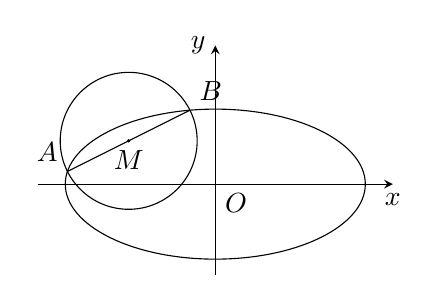
\begin{tikzpicture}[scale=0.55,>=stealth]
  \draw[->] (-4.1,0)--(4.1,0) node[below] {$x$};
  \draw[->] (0,-2.1)--(0,3.2) node[left] {$y$};
  \draw (0,0) ellipse ({sqrt(12)} and {sqrt(3)});
  \draw (-2,1) circle ({sqrt(2.5)});
  \coordinate (A) at ({-2-sqrt(2)},{1-sqrt(0.5)});
  \coordinate (B) at ({-2+sqrt(2)},{1+sqrt(0.5)});
  \draw (A)--(B);
  \fill (-2,1) circle (1.2pt);
  \node[above left] at (A) {$A$};
  \node[above right] at (B) {$B$};
  \node[below] at (-2,1) {$M$};
  \node[below right] at (0,0) {$O$};
\end{tikzpicture}
